\documentclass[a4paper]{article}
\usepackage[utf8]{inputenc}
\usepackage[russian]{babel}
\usepackage[T2]{fontenc}
\usepackage[warn]{mathtext}
\usepackage{graphicx}
\usepackage{amsmath}
\usepackage{floatflt}
\usepackage[left=20mm, top=20mm, right=20mm, bottom=20mm, footskip=10mm]{geometry}


\graphicspath{ {images/} }
\usepackage{multicol}
\setlength{\columnsep}{2cm}
\author{Данакари Никита, Б03-103} 
\date{13 сентября 2023 г.}
\title{\textbf{Работа 8.1\\
Тепловое Излучение}}
\newtheorem{task}{Задача}
\newtheorem{zam}{Замечание}
\begin{document}
\maketitle
\section{Аннотация}

\par В данной работе было исследовано тепловое излучение различных тел с помощью оптического пирометра. Наблюдались тела с различной яркостной температурой, но одинаковой термодинамической. Исследована модель АЧТ. Оценены значения констант Стефана-Больцмана и Планка.
\section{Оборудование}
Пирометр,  модель  АЧТ,  термопара,  трубка  с  кольцами  из 
материалов с различной испускательной  способностью, лампа накаливания, неоновая 
лампочка, вольтметр, амперметр.

\section{Теоретические положения}
Для измерения температуры разогретых тел, удалённых от наблюдателя, применяют методы оптической пирометрии, основанные на использовании зависимости испускательной способности исследуемого тела от температуры. Различают три температуры, функционально связанные с истинной термодинамической температурой и излучательной способностью тела: радиационную $T_{rad}$, цветовую $T_{col}$ и яркостную $T_b_r$. \par
В данной работе измеряется яркостная температура. \textbf{Яркостная температура} - это температура абсолютно чёрного тела, при которой его спектральная испускательная способность равна спектральной испускательной способности исследуемого тела при той же длине волны.
 Измерение яркостной температуры раскалённого тела производится при помощи оптического пирометра с исчезающей нитью, основанного на визуальном сравнении яркости раскалённой нити с яркостью изображения исследуемого тела. \par
Яркостная температура тела всегда ниже его термодинамической температуры. Это связано с тем, что любое нечёрное тело излучает меньше, чем АЧТ при той же температуре. Зависимость между яркостной и термодинамической температурами вольфрама приведена на рис. 1

\begin{figure}[h]
    \centering
    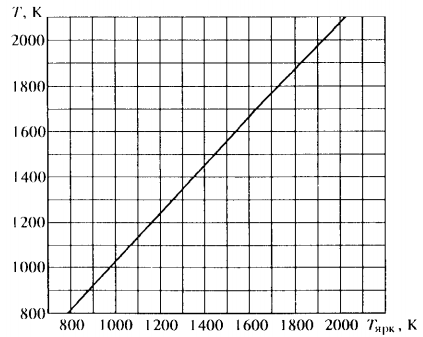
\includegraphics[width=10cm]{fig2.PNG}
    \caption{График зависимости $T = f(T_b_r)$ для вольфрам}
    \label{fig:vac}
\end{figure}

По результатам измерений мощности излучения вольфрамовой нити можно судить о справедливости закона Стефана-Больцмана. Если бы нить излучала как АЧТ, то баланс потребляемой и излучаемой энергии определялся бы соотношением 
\begin{equation}
    W = \sigma S (T^4 - T_0^4),
\end{equation}
где $W$ - потребляемая нитью электрическая мощность, $S$ - площадь излучающей поверхности нити, $T$ - температура нити, $T_0$ - температура окружающей среды. Однако вольфрамовая нить излучает как серое тело, и излучение её ослаблено по сравнению с АЧТ в $\varepsilon_T$ раз для любой волны при данной температуре тела Т. Тогда предположив, что нить излучает как серое тело и с учётом того, что $T_0 \ll T$, выражение (1) можно переписать в виде
\begin{equation}
    W = \varepsilon_T S \sigma T^4
\end{equation}
В справедливости закона Стефана-Больцмана можно убедиться, построив график зависимости $W(T)$ в логарифмическом масштабе, и по углу наклона определить показатель степени $n$ исследуемой температурной зависимости. В пределах погрешности показатель степени должен быть близок к четырём. \par
Также из формулы (2) можно определить постоянную Стефана-Больцмана.

\newpage

\section{Экспериментальная установка}

\begin{figure}[h]
    \centering
    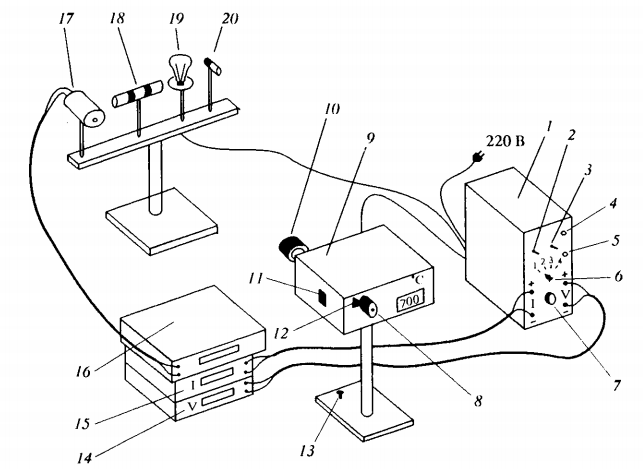
\includegraphics[width=11cm]{fig1.PNG}
    \caption{Схема экспериментальной установки: 1 - блок питания; 2 - тумблер включения питания образцов; 3 - тумблер нагрева нити пирометра; 4 - кнопка "Нагрев нити"; 5 - кнопка "охлаждение нити"; 6 - тумблер переключения образцов; 7 - регулятор мощности нагрева образцов; 8 - окуляр пирометра; 9 - корпус пирометра; 10 - объектив пирометра; 11 - переключение диапазонов; 12 - ручка смещения красного светофильтра; 13 - регулировочный винт; 14 - вольтметр (напряжение на лампе накаливания); 15 - амперметр (ток через образцы); 16 - вольтметр в цепи термопары; 17 - модель АЧТ; 18 трубка с кольцами из материалов с различной излучательной способностью; 19 - лампа накаливания; 20 - неоновая лампочка}
    \label{fig:vac}
\end{figure}

Исследуемые в работе образцы:
\begin{itemize}
    \item \textbf{модель абсолютно чёрного тела} - керамическая трубка, закрытая с одного конца и окружённая для теплоизоляции внешним кожухом. Температура в трубке измеряется с помощью термопары хромель-алюмель
    \item \textbf{керамическая трубка с набором колец из различных материалов}, нагреваемая изнутри нихромовой спиралью. Материалы колец имеют различную излучательную способность
    \item \textbf{вольфрамовая нить электрической лампочки}
\end{itemize}

\newpage

\section{Ход работы}
\subsection{Изучение работы оптического пирометра}

Определим по шкале пирометра значение яркостной температуры модели АЧТ. Одновременно измерим температуру модели АЧТ при помощи хромельалюмилевой термопары и цифрового вольтметра.
Значения температуры, полученные обоими способами, мало отличаются друг от друга, схожи в пределах 5\%, следовательно, пирометр работает исправно. \\\\
\subsection{Измерение яркостной температуры тел}\\
Нагреем трубку до темно-красного каления (900 $^\circ$C) и визуально измерим яркостную температуру ее поверхности, а также правого и левого кольца.

Кольца и трубка излучают разное количество света. Это обусловлено тем, что материалы, из которых изготовлены кольца, излучают не так, как АЧТ, и тем, что разные материалы имеют различную испускательную способность.

\newpage
\subsection{Проверка закона Стефана-Больцмана}
    \par Постепенно увеличивая накал нити лампы, начиная со слабого тёмно-красного накала до 1940$^{\circ}$C, будем измерять пирометром яркостную температуру нити, а также значение силы тока и напряжения на ней. Результаты измерений занесём в таблицу 1. Определим также по значениям яркостной температуры нити её термодинамическую температуру, используя рис. 1.
    


Для проверки закона Стефана-Больцмана построим в логарифмическом масштабе график зависимости $\ln(T)=g(W)=k\ln(W) + c$, так как погрешность по температуре много больше погрешности мощности. Тогда получим 

\begin{figure}[h]
    \centering
    \includegraphics[width=10cm]{Capture.PNG}
    \caption{график зависимости $\ln(T)=g(W)=k\ln(W) + c$}
    \label{fig:vac}
\end{figure}

Получим значения коэффициентов:
$$k=0.261\pm0.006$$
$$c=3.108\pm0.003$$
\par Откуда рассчитаем значения коэффициентов для искомой прямой $\ln(W)=n\ln(T)+b$:
$$n=\frac{1}{k}=3.83\pm0.08$$
$$b=-\frac{c}{k}=-11.9\pm0.2$$
\par Полученное значение $n$ близко к четырём, что подтверждает закон Стефана-Больцмана

Для каждого измеренного значения $T$, превышающего 1700К найдем величину постоянной Стефана-Больцмана, и, зная ее, найдем постоянную Планка:
\[
\sigma = \frac{W}{\xi_T S T^4}, \hspace{10pt} \sigma_\sigma = 4\sigma_T \hspace{40pt} h = (\frac{2 \pi^5 k^4_\text{Б}}{15c^2 \sigma})^{1/3}, \hspace{10pt} \sigma_h = \frac{4}{3} \sigma_T
\]

    \begin{table}[h]
    \centering
    \begin{center}
    \caption{Определение значений постоянной Стефана-Больцмана $\sigma$ и Планка $h$ и их погрешностей.}
    \end{center}
\begin{tabular}{|l|l|l|l|l|l|l|l|}
\hline
$T$,$^{\circ}$C & $T$, K & $\varepsilon_T$ & $W$, мВт    & $\sigma$, $10^{-8}$ Дж*с$^{-1}$*м$^{-2}$*K$^{-4}$ & $\sigma_\sigma$, $10^{-8}[\sigma]$ & $h$, $10^{-34}$ Дж*с    & $\sigma_h$, $10^{-34}$ $[h]$  \\ \hline
1560 & 1833 & 0.195   & 3.94 & 4.97  & 0.99         & 7.05 & 0.47     \\ \hline
1665 & 1938 & 0.209   & 5.00 & 4.72  & 0.94         & 7.17 & 0.48     \\ \hline
1770 & 2043 & 0.223   & 5.75 & 4.11  & 0.82         & 7.51 & 0.50     \\ \hline
1875 & 2148 & 0.236   & 7.05 & 3.90  & 0.78         & 7.65 & 0.51     \\ \hline
1980 & 2253 & 0.249   & 8.52 & 3.69  & 0.74         & 7.79 & 0.52     \\ \hline
\end{tabular}
\end{table}   

\begin{center}
 Табличные значения:\\
$\sigma_t_h = 5.67\cdot 10^{-8}$ Дж*с$^{-1}$*м$^{-2}$*K$^{-4}$ \\
$h_t_h = 6.62\cdot 10^{-34}$ Дж*с
\end{center}
\subsection{Измерение яркостной температуры неоновой лампочки}
«Яркостная температура» неоновой лампочки, измеренная с помощью пирометра, 
равна 860°С При этом термодинамическая температура лампочки равняется нескольким 
десяткам градусов Цельсия. Это вызвано тем, что лампа излучает не так, как АЧТ, а ее яркость вызвана газовыми разрядами (электроны переходят с резонансного уровня на нейтральный, при этом излучая фотоны).
\section{Вывод}
В ходе работы была изучена модель абсолютно черного тела.
Было показано, что  различные  тела, накаленные  до  одинаковой  термодинамической 
температуры, могут иметь различную яркостную температуру. Проверен закон Стефана-Больцмана. Рассчитана постоянная Стефана-Больцмана. Рассчитана постоянная Планка. Все полученные значения сходятся с табличными в пределах погрешности.
\end{document}